\subsubsection{pr05}
\label{subsubsec:pr05}
The obtained results were the following:
{
\renewcommand{\arraystretch}{2}
\begin{longtable}[h]{| c | c | c | c | c |}
    \hline
    \textbf{Failures} & \multicolumn{3}{c}{Time limit} & \\
    \hline
    \textbf{Search strategy} & \textbf{\textit{30 sec}} & \textbf{\textit{1 min}} & \textbf{\textit{2 min}} & \textbf{\textit{5 min}} \\
    \hline
    \endhead
    default search                                         & 148 &  148 &  5.032 &  14.801 \\
    \hline
    domWdeg, random                                        &  73 &   73 &  4.956 &  14.722 \\
    \hline
    domWdeg, random, Luby restart L=250                    & 100 &  100 &   100 &    450 \\
    \hline
    \textit{domWdeg, random, Luby restart L=250, LNS 85\%} & 100 &  100 &   100 &    136 \\
    \hline
    domWdeg, random, Luby restart L=250, LNS 15\%          & 100 &  100 &   612 &   4.389 \\
    \hline
    first fail, min                                        &  16 &   16 &  4.900 &   9.785 \\
    \hline
\end{longtable}
}
\begin{figure}[H]
    \centering
    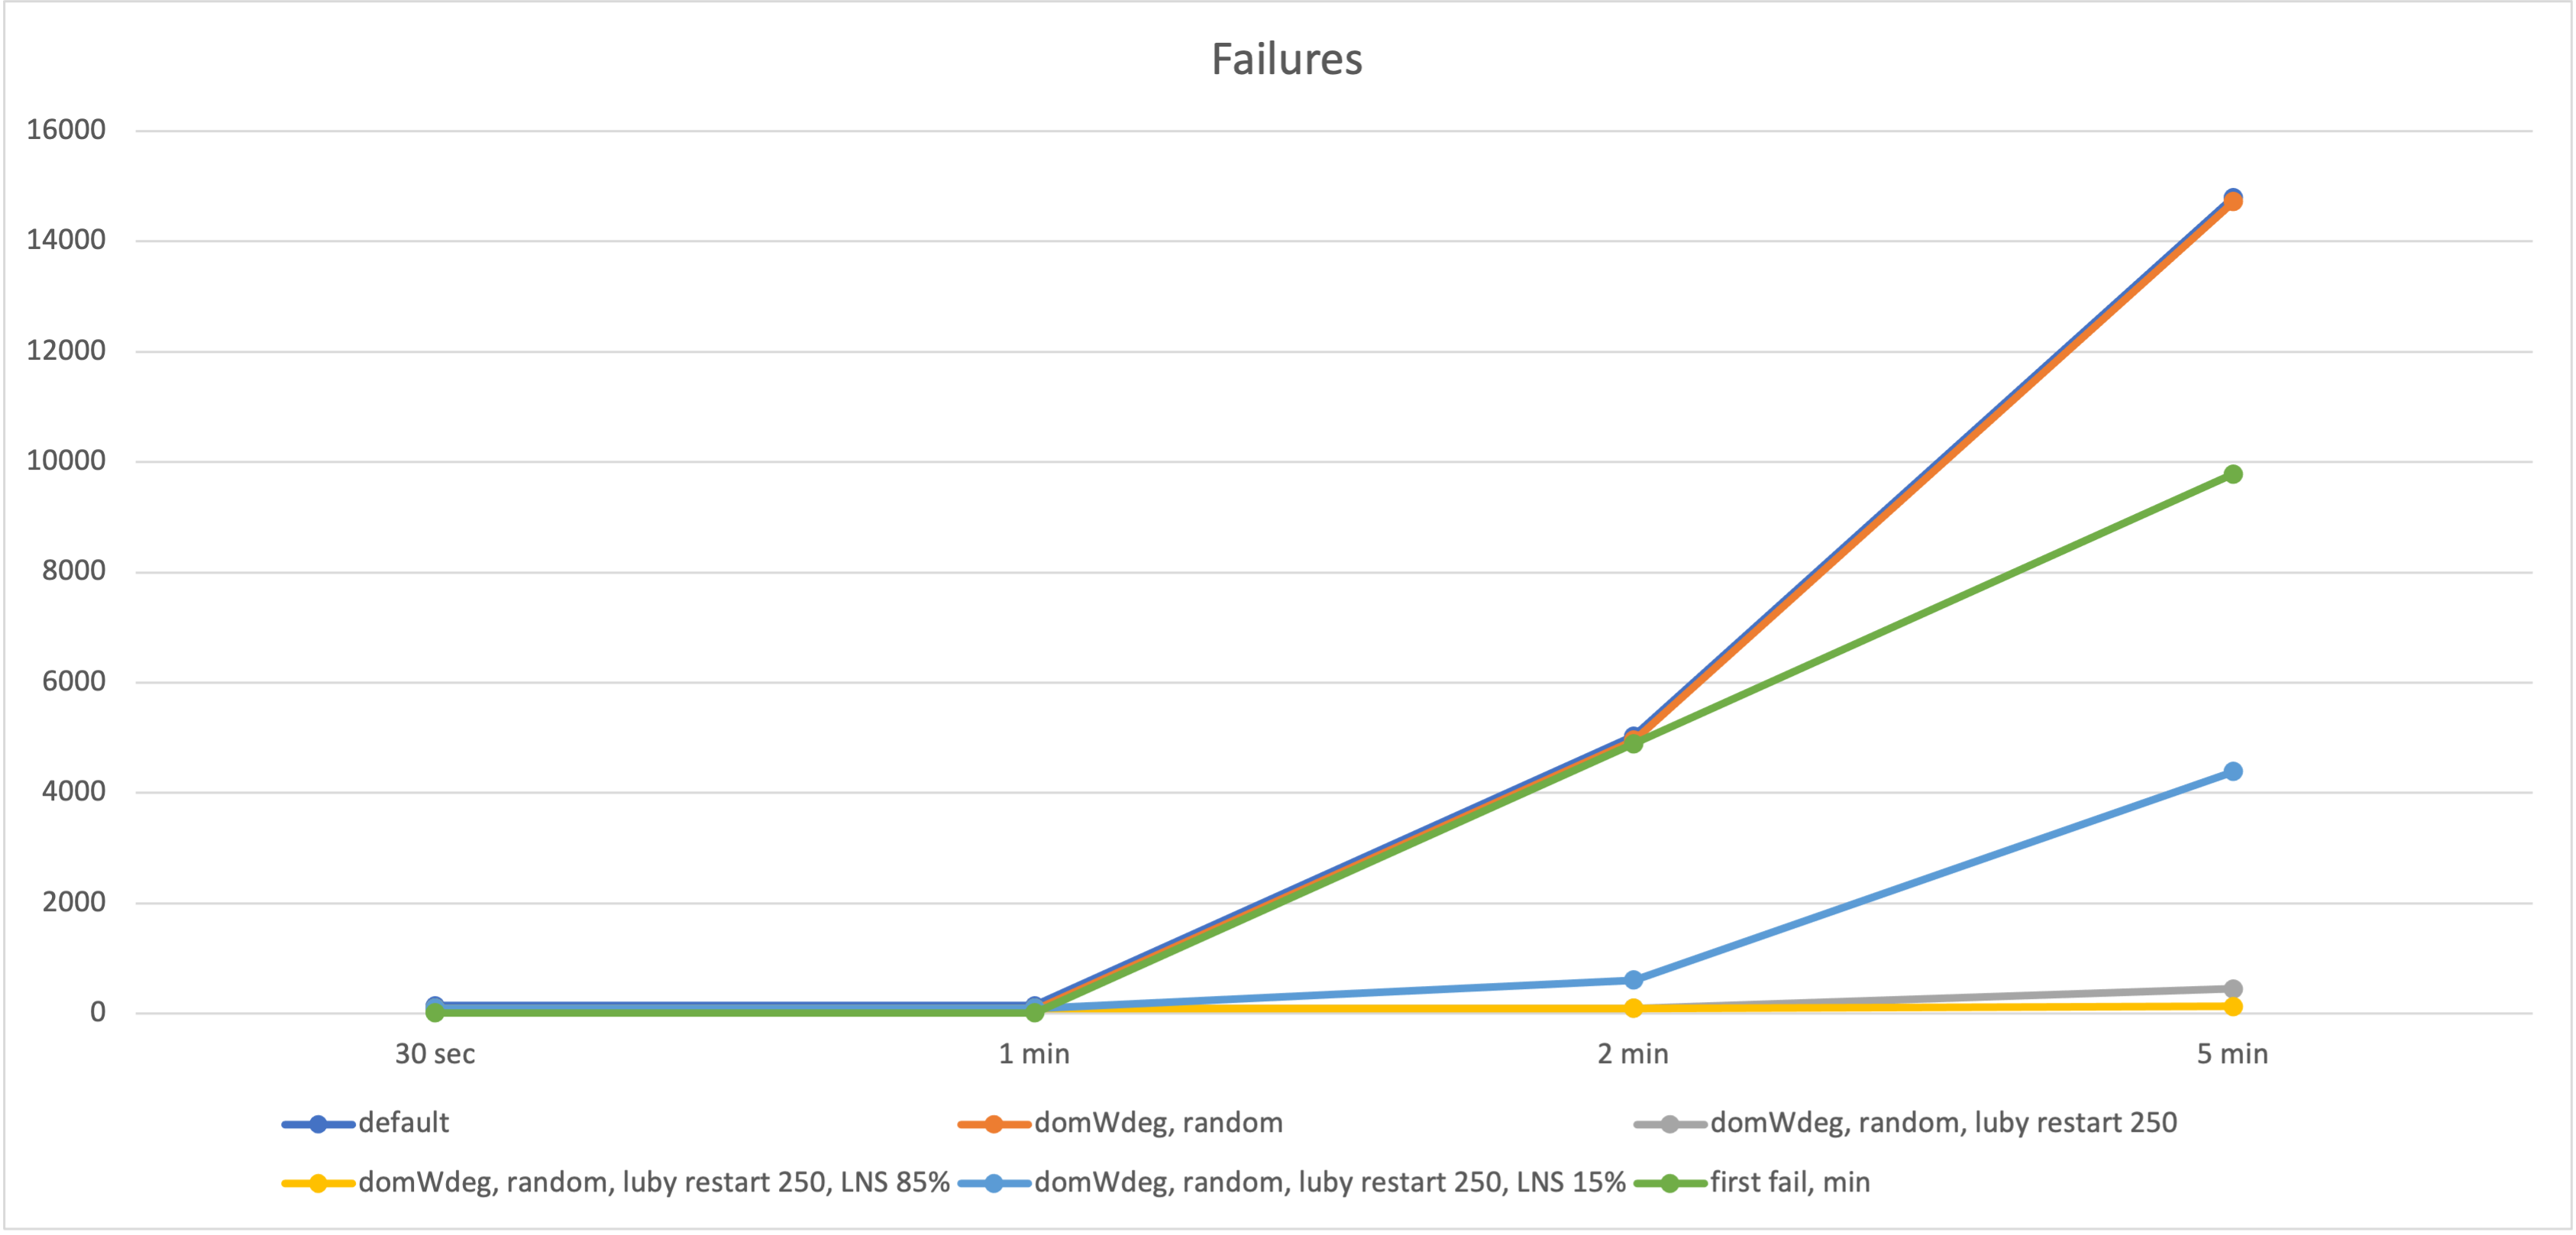
\includegraphics[width=0.8\columnwidth]{../graphs/pr05-failures.png}
    \caption{Failures graph for \textbf{pr05}.}
\end{figure}

{
\renewcommand{\arraystretch}{2}
\begin{longtable}[h]{| c | c | c | c | c |}
    \hline
    \textbf{Objective function} & \multicolumn{3}{c}{Time limit} & \\
    \hline
    \textbf{Search strategy} & \textbf{\textit{30 sec}} & \textbf{\textit{1 min}} & \textbf{\textit{2 min}} & \textbf{\textit{5 min}} \\
    \hline
    \endhead
    default search                                        & - & - & 149.075.130 & 148.726.590 \\
    \hline
    domWdeg, random                                       & - & - & 152.915.400 & 152.300.890 \\
    \hline
    domWdeg, random, Luby restart L=250                   & - & - & 146.190.950 & 145.542.940 \\
    \hline
    domWdeg, random, Luby restart L=250, LNS 85\%         & - & - & 146.190.950 & 144.986.790 \\
    \hline
    domWdeg, random, Luby restart L=250, LNS 15\%         & - & - & 146.190.950 & 145.472.140 \\
    \hline
    \textit{first fail, min}                              & - & - & 140.606.490 & 140.547.390 \\
    \hline
\end{longtable}
}
\begin{figure}[H]
    \centering
    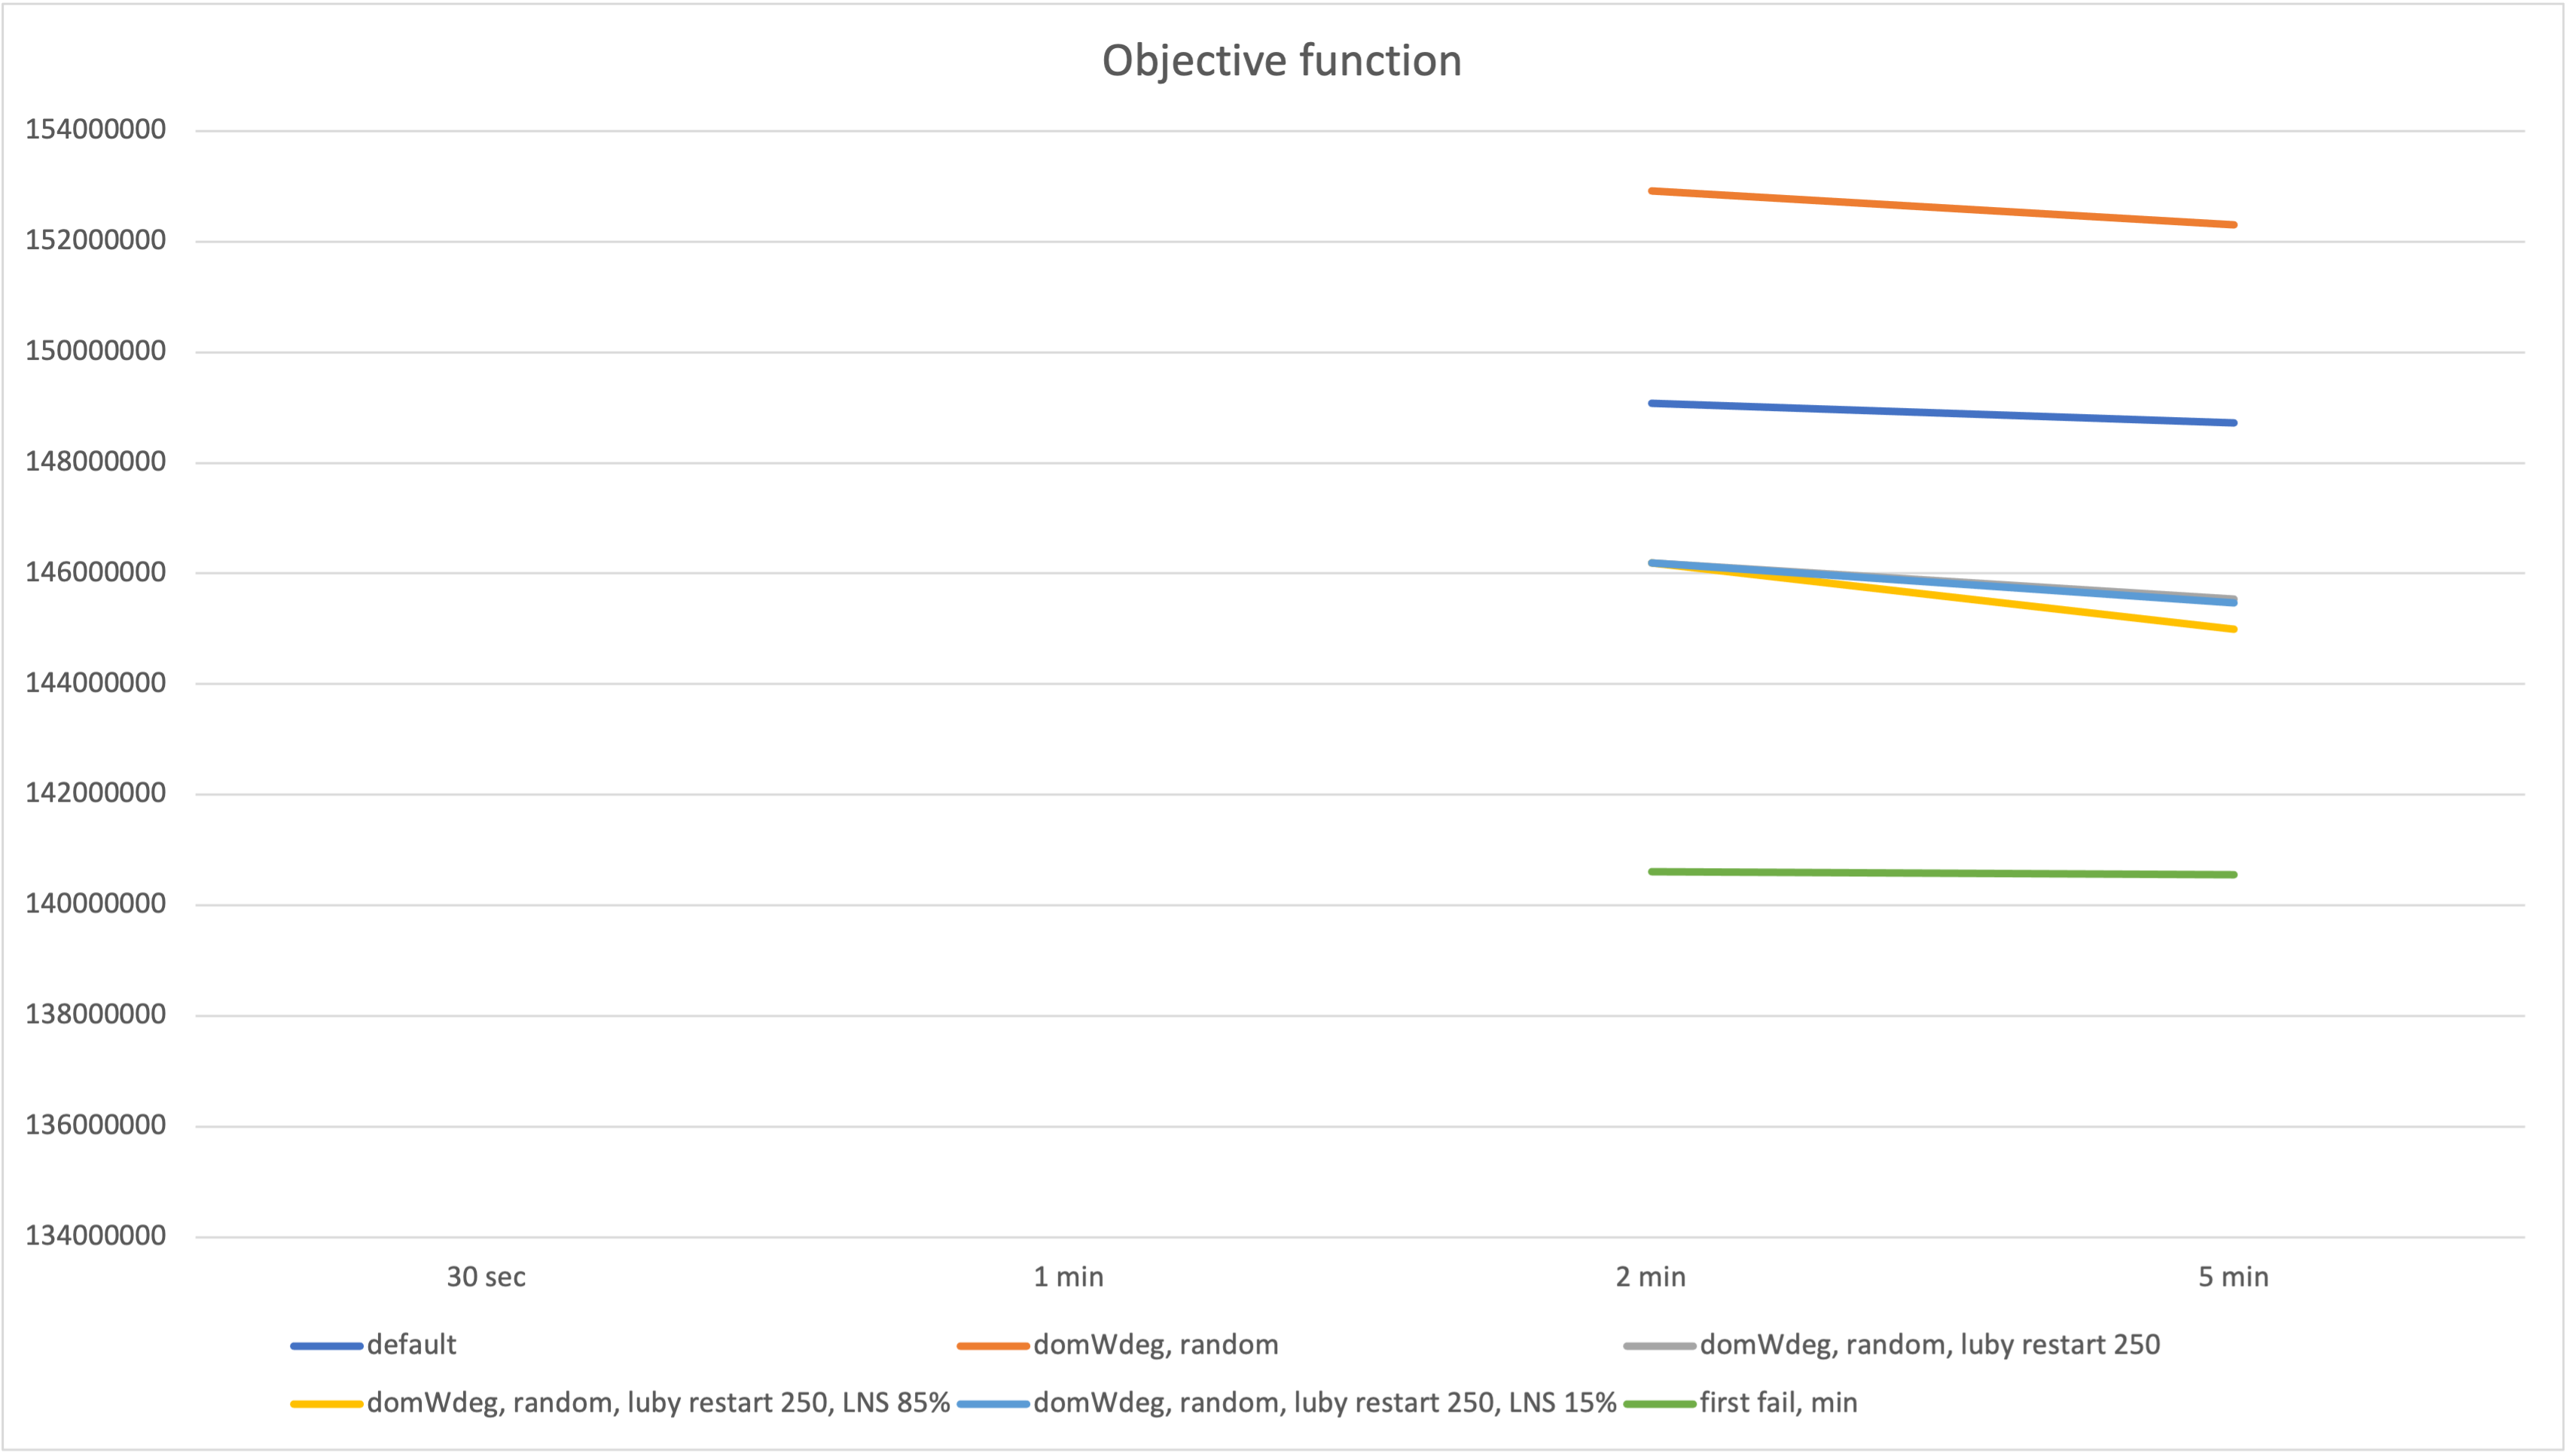
\includegraphics[width=0.8\columnwidth]{../graphs/pr05-objf.png}
    \caption{Objective functions graph for \textbf{pr05}.}
\end{figure}

{
\renewcommand{\arraystretch}{2}
\begin{longtable}[h]{| c | c | c | c |}
    \hline
    \textbf{Weights} & \textbf{Objective function} & \textbf{Total distance} & \textbf{Used vehicles} \\
    \hline
    \endhead
    $\alpha = 10, \beta = 0$ & 144.930.250 & 14.493.025 & 20 \\
    \hline
    $\alpha = 7, \beta = 3$  & 101.451.235 & 14.493.025 & 20 \\
    \hline
    $\alpha = 5, \beta = 5$  &  72.465.225 & 14.493.025 & 20 \\
    \hline
    $\alpha = 3, \beta = 7$  &  43.483.985 & 14.494.615 & 20 \\
    \hline
    $\alpha = 0, \beta = 10$ &         200 & 14.619.095 & 20 \\
    \hline
\end{longtable}
}
\begin{figure}[H]
    \centering
    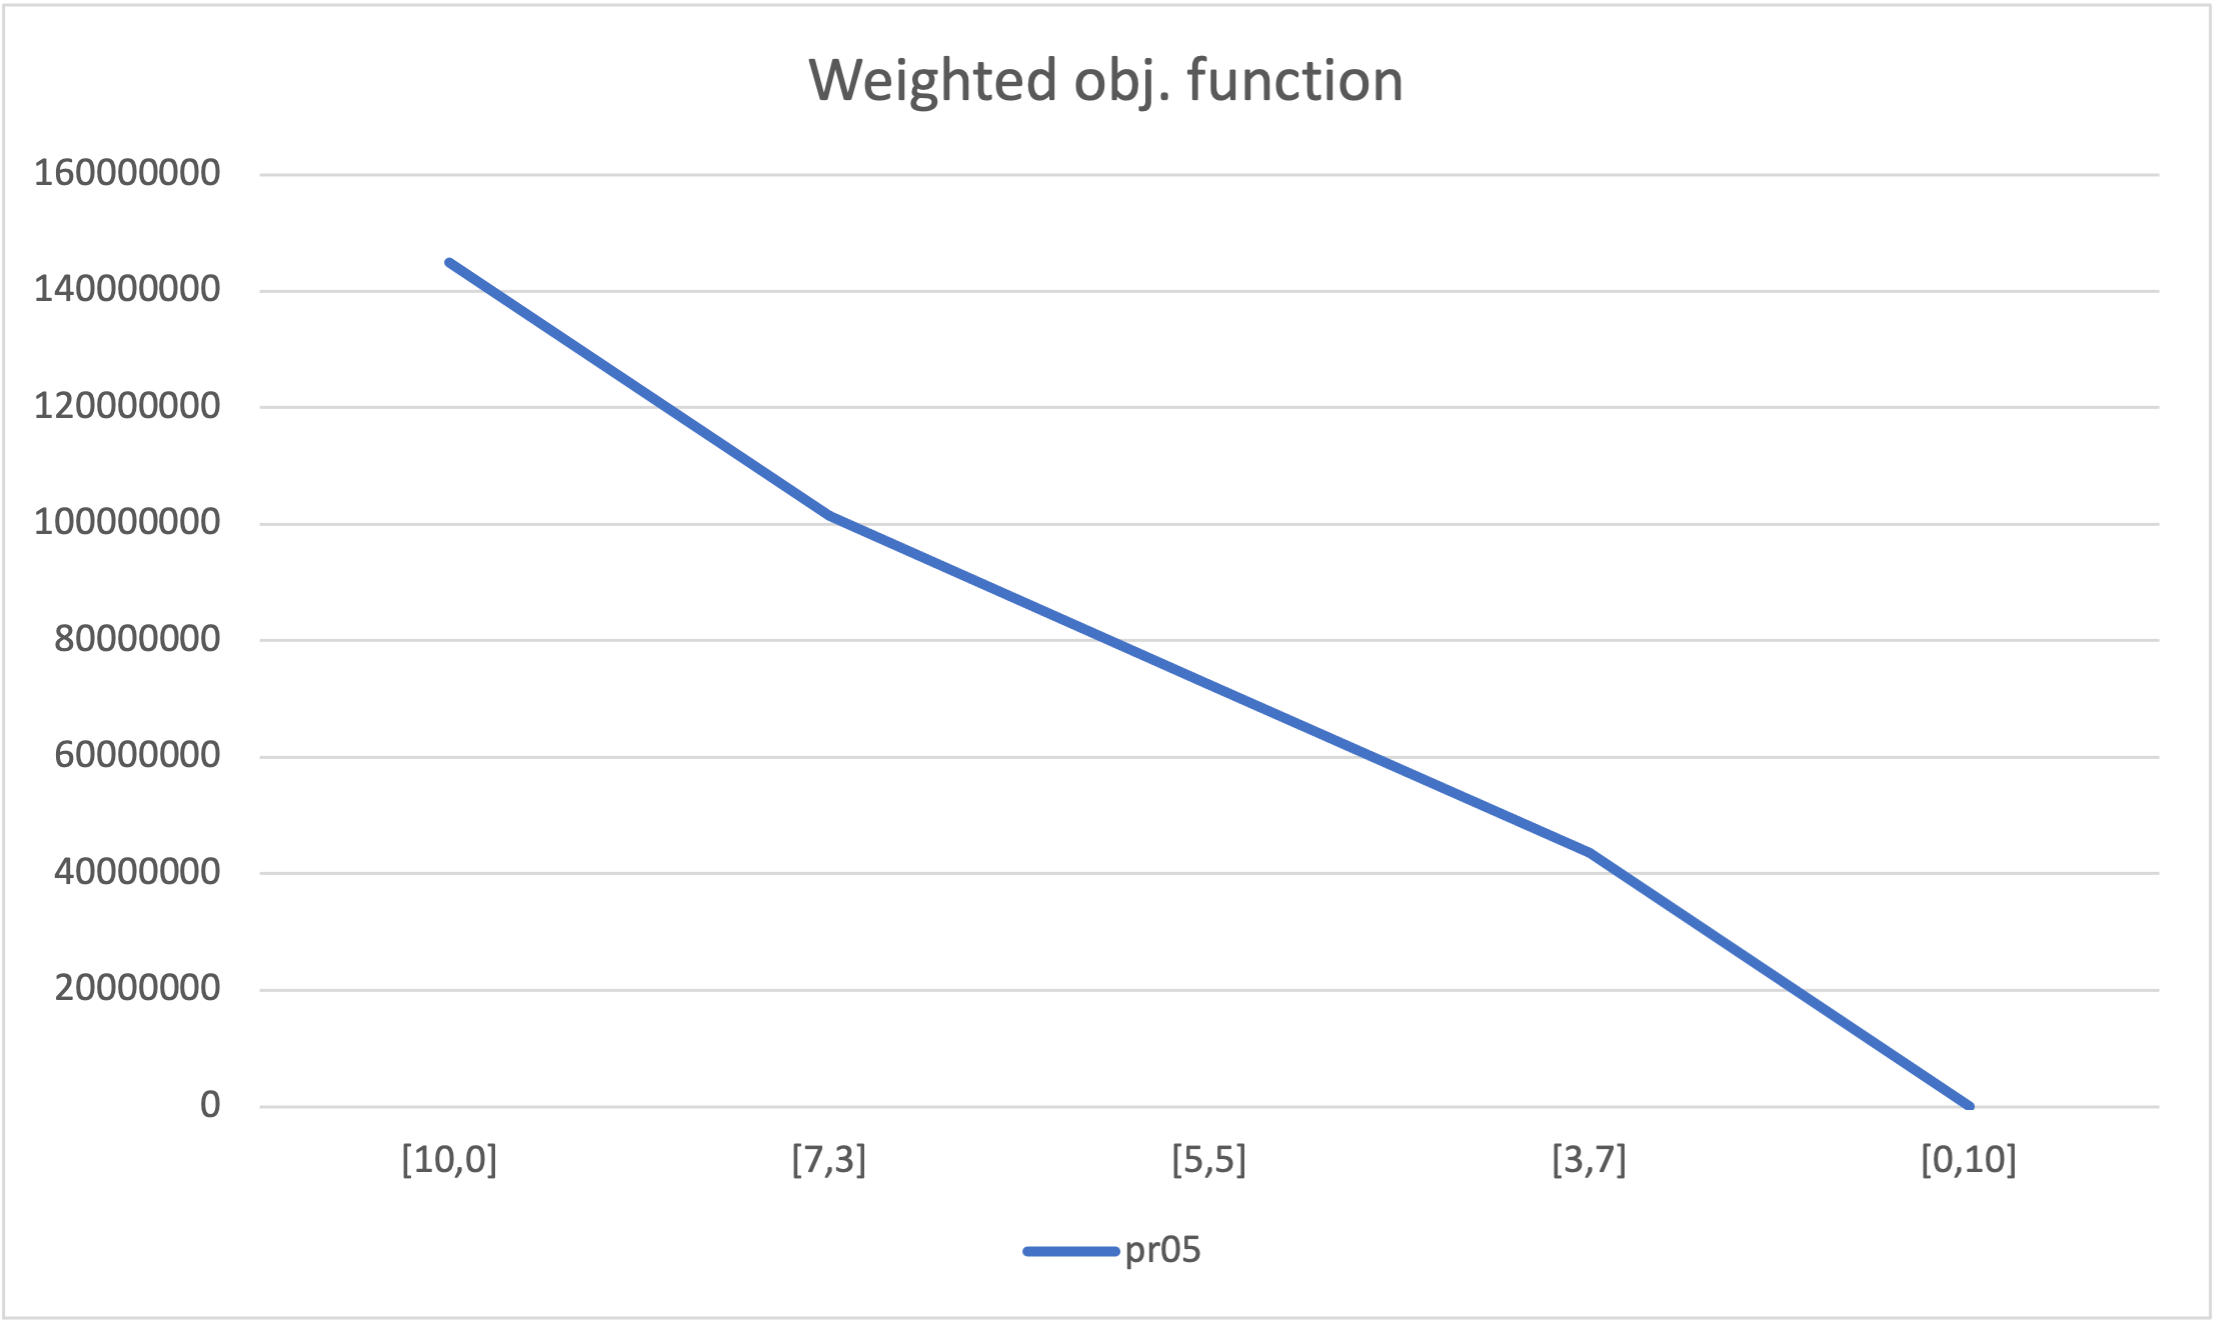
\includegraphics[height=0.25\textheight]{../graphs/pr05-wobjf.png}
    \caption{Weighted objective functions graph for \textbf{pr05}.}
\end{figure}

\begin{figure}[H]
    \centering
    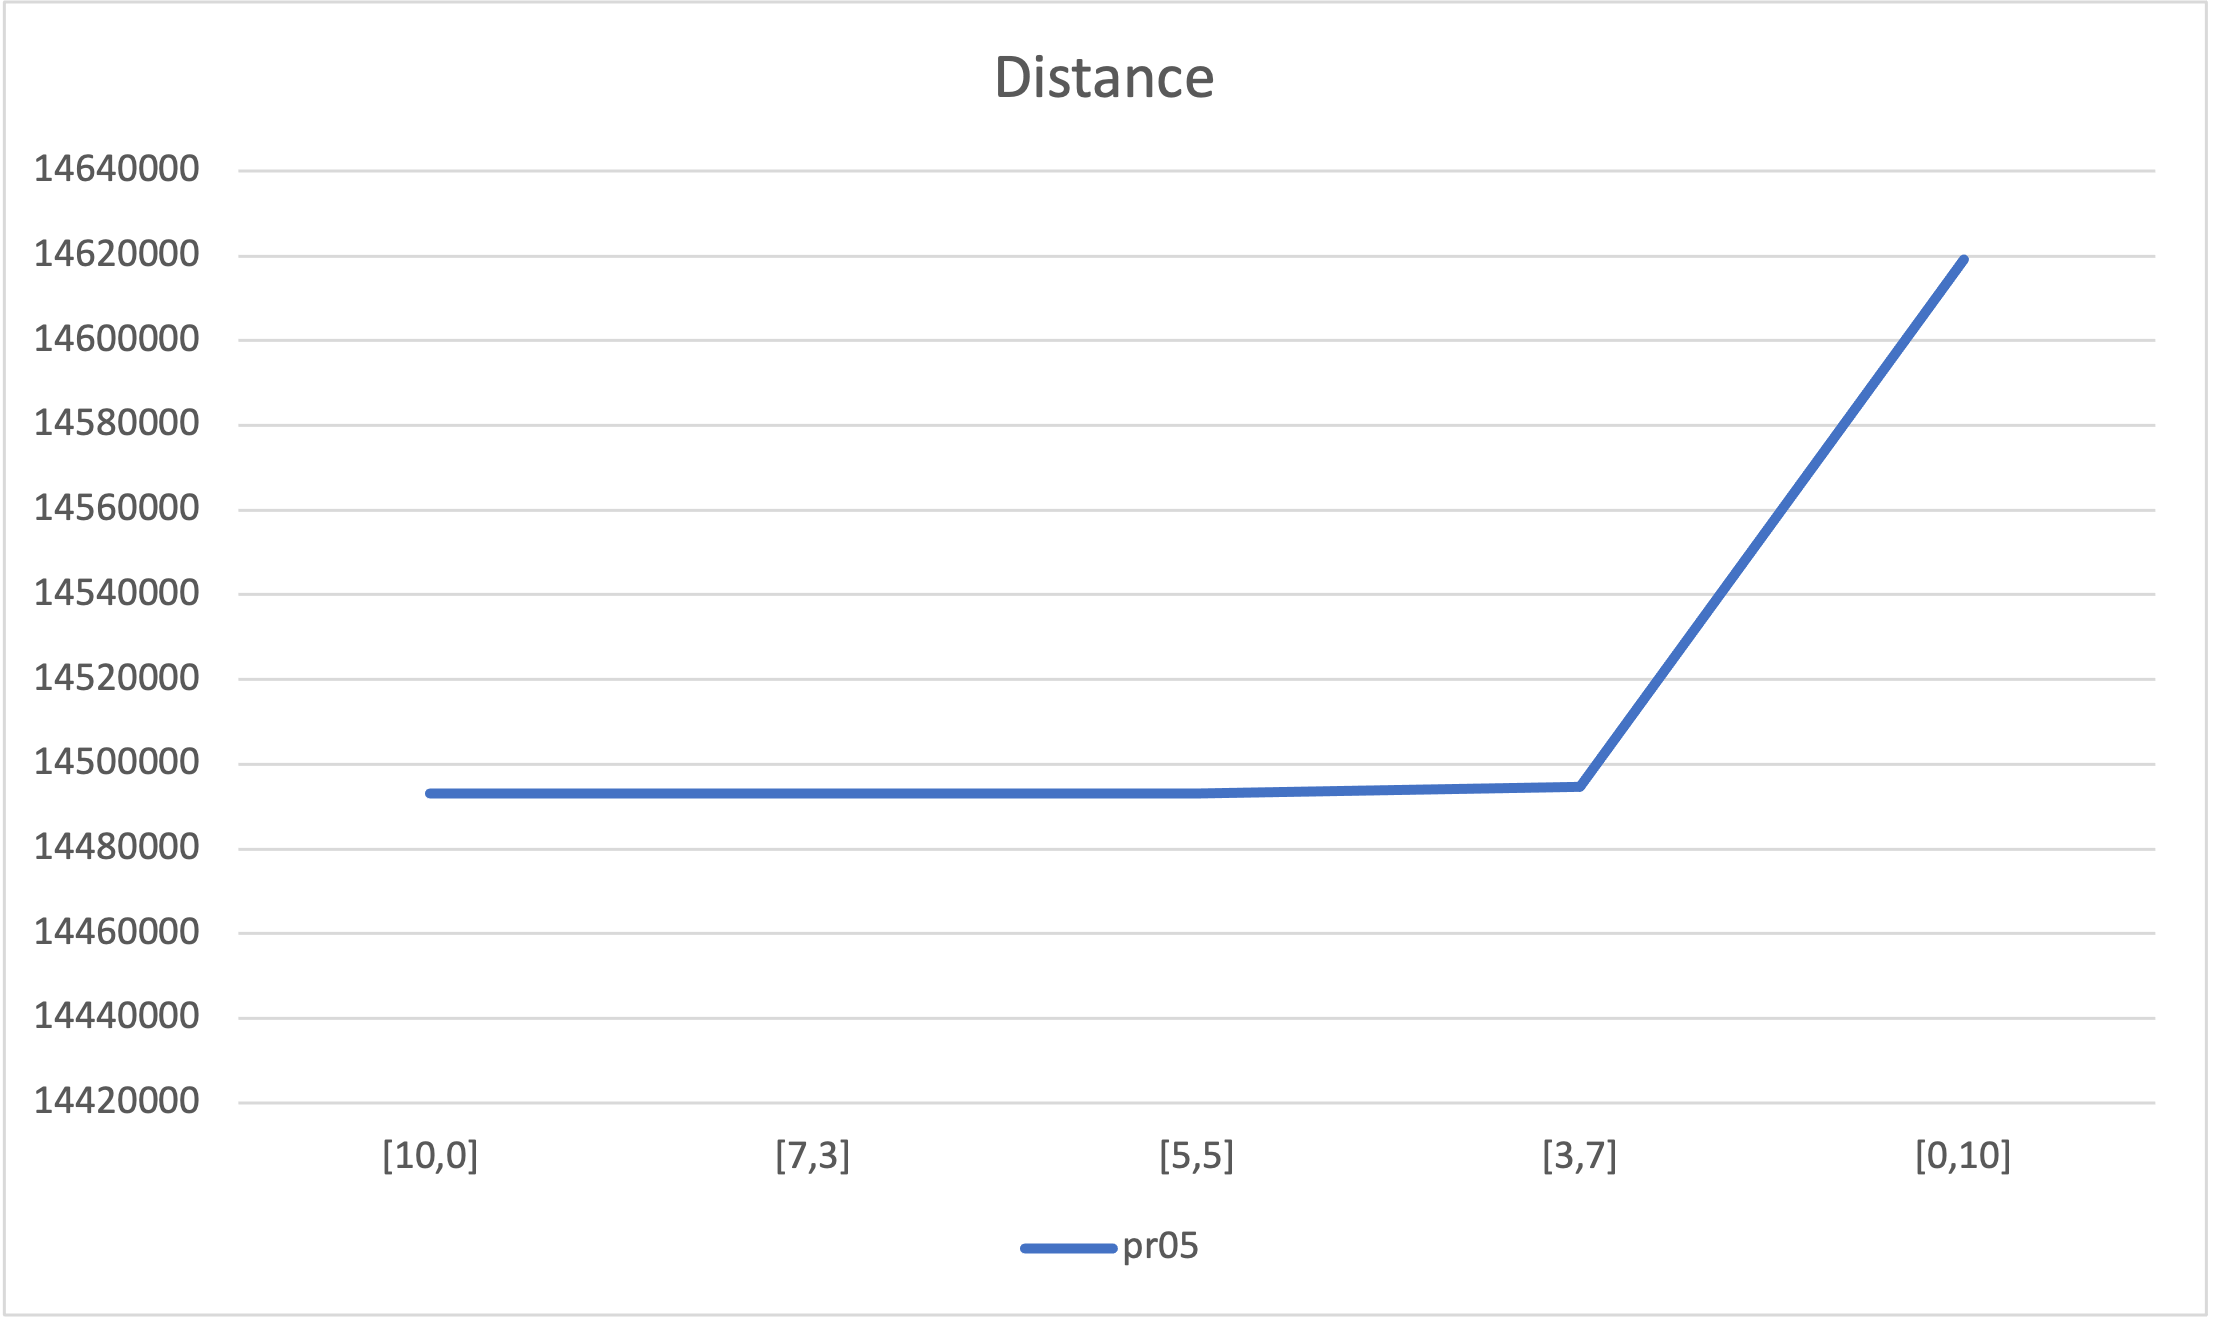
\includegraphics[height=0.25\textheight]{../graphs/pr05-distance.png}
    \caption{Distances graph for \textbf{pr05}.}
\end{figure}

\begin{figure}[H]
    \centering
    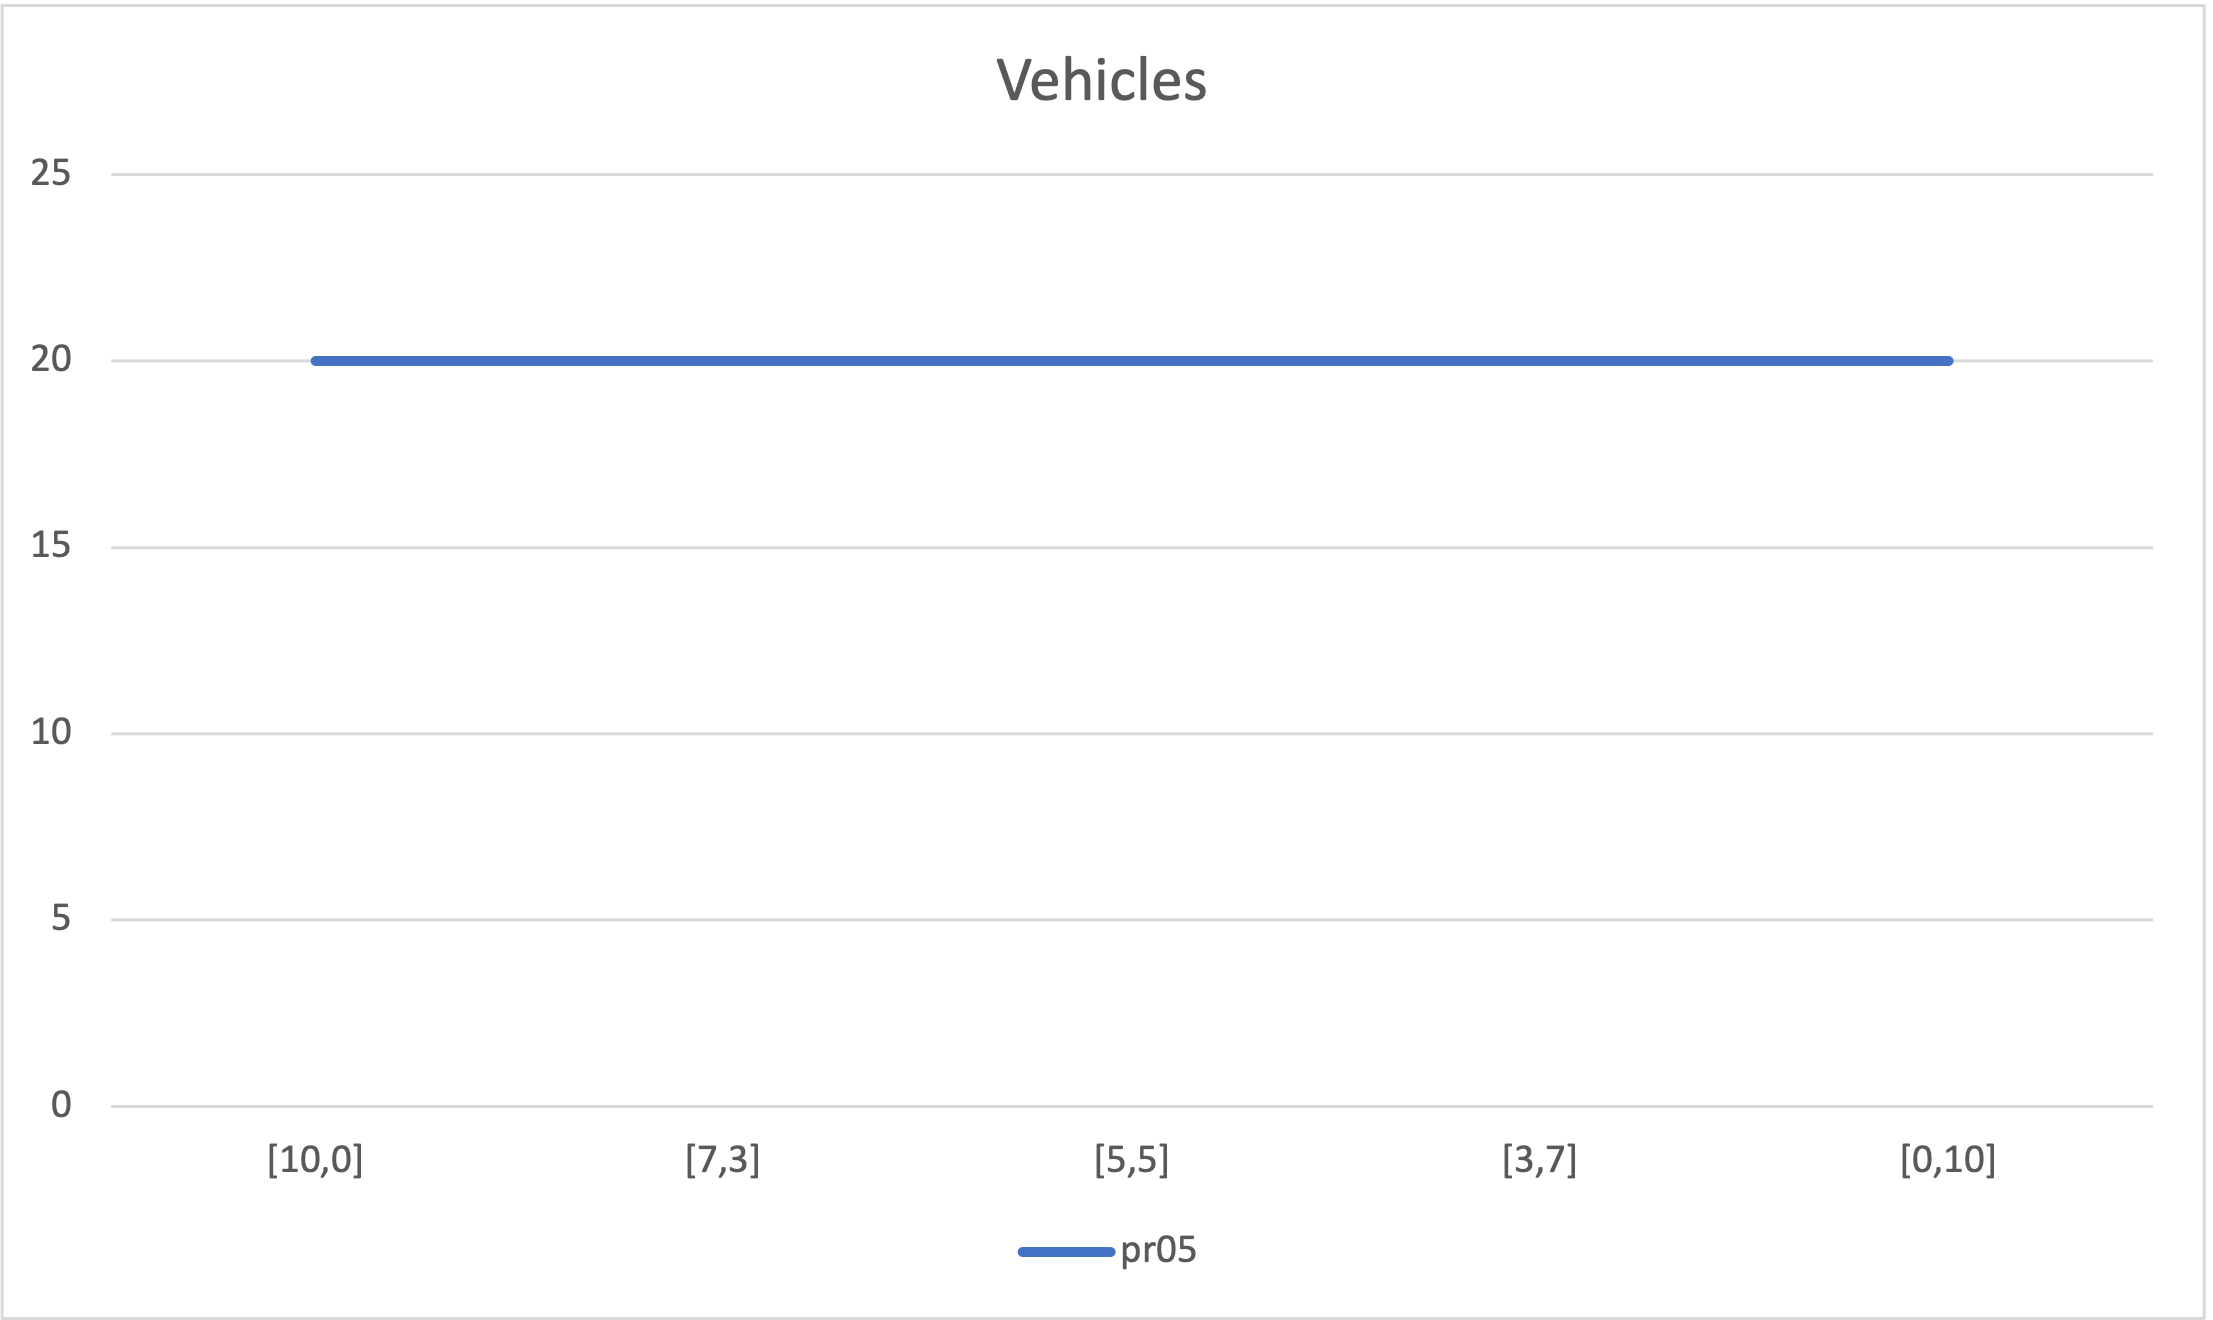
\includegraphics[height=0.25\textheight]{../graphs/pr05-vehicles.png}
    \caption{Vehicles used graph for \textbf{pr05}.}
\end{figure}

\newpage
